\documentclass{article}
\usepackage{tikz}
\usepackage{amsmath}
\usepackage{array}
\usepackage{listings}
\usepackage{csvsimple}
\usepackage{booktabs}
\usepackage{float}
\usepackage{hyperref}
\usepackage{makeidx}
\usetikzlibrary{positioning,chains,fit,shapes,calc}
\usetikzlibrary{positioning,chains,fit,shapes,decorations.pathreplacing}

\usepackage[ruled,linesnumbered]{algorithm2e}
\makeindex
\title{GRASP-Based Approach to the Course Faculty Assignment Problem}
\author{
  \textnormal{Jainam Shah } \cdot \textnormal{ Michael Lewis } \cdot \textnormal{ Mahir Jimit Ghadiali}
}
\date{November 2023}

\definecolor{myblue}{RGB}{80,80,160}
\definecolor{mygreen}{RGB}{80,160,80}

\begin{document}

\maketitle

\index{Introduction}
\section{Introduction}
The focal point of our research revolves around optimizing the University Course Assignment System. Within a department, faculty members are classified into three distinct groups: $x_1$, $x_2$, and $x_3$. Each group has a designated maximum course load, with $x_1$ handling 0.5 courses per semester, $x_2$ managing 1 course per semester, and $x_3$ overseeing 1.5 courses per semester.
\par
This system allows faculty members the flexibility to enroll in multiple courses during a semester, and conversely, a single course may be assigned to multiple faculty members. When a course is shared between two professors, each professor's load is considered to be 0.5 courses. Additionally, each faculty member maintains a preference list of courses, ordered by personal preference, with the most favored courses listed at the top. It is important to note that there is no prioritization among faculty members within the same category.
\par
The primary objective of this research problem is to devise an assignment scheme that maximizes the number of courses assigned to faculty while adhering to their preferences and the category-based constraints ($x_1$, $x_2$, $x_3$). The challenge lies in ensuring that a course can only be assigned to a faculty member if it is present in their preference list. Also among the courses, the CDCs(Compulsory Disciplinary Courses) have higher priority to be assigned than the Electives. So the algorithm must assign all CDCs (unless not possible) while also maximising the total number of courses assigned.
\par
This problem stands out due to the flexibility it offers regarding the number of courses faculty members can undertake, setting it apart from typical Assignment problems. Also keeping the preference of the faculties in mind while giving multiple sub optimal solutions is required so that the Department HOD can make the last call by choosing 1 among the possible solutions. Possible modifications may involve adjusting the maximum number of courses $y$ for each category of professors, rather than requiring strict adherence, or expanding the number of professor categories beyond the existing three to create a more generalized solution.

\newpage
\index{Problem Constraints and Assumptions}
\section{Problem Constraints and Assumptions}

\subsection{Hard Constraints}

The formulation of the University Course Assignment Problem is bound by the following hard constraints:

\begin{enumerate}
    \item \textbf{Maximum Course Load:} The maximum course load for each faculty member must be maintained, distinguishing between three categories: $x_1$, $x_2$, and $x_3$, representing 0.5, 1, and 1.5 courses per semester, respectively.
    
    \item \textbf{Faculty Assignment to Courses:} Each course should have either 1 or 2 faculty members assigned to it. This ensures that a course is either solely assigned to one faculty or shared between two.
    
    \item \textbf{Complete Assignment:} A course should not remain partially assigned. For shared courses, it must be assigned to exactly 2 faculties, maintaining completeness in faculty assignment.
    
    \item \textbf{CDC Assignment:} All Compulsory Disciplinary Courses (CDCs) must be assigned if possible. Priority is given to ensure the assignment of all CDCs.
\end{enumerate}

\subsection{Soft Constraints}

The soft constraints, while not mandatory, add additional considerations for optimizing the assignment process:

\begin{enumerate}
    \item \textbf{Teacher's Course Preferences:} Faculty members' course preferences should be taken into account during the assignment process. This involves considering the ordered lists of courses provided by each faculty member.
    
    \item \textbf{Balanced Course Load:} The course load of faculty members should be balanced across all teachers as much as possible. This soft constraint aims to distribute the workload evenly among faculty members.
\end{enumerate}

\subsection{Assumptions}

Certain assumptions have been made to facilitate the formulation of the problem:

\begin{enumerate}
    \item \textbf{Equal Preference Priority:} In cases where multiple faculty members have the same position in the preference list for a particular course, there is no preference given to one professor over another. This assumption ensures fairness in course assignments.
\end{enumerate}
\newpage
\index{Objective Function}
\section{Objective Function}

The objective function for the problem is as follows:


    \begin{equation}
\text{Maximize } \sum_{i} \mathit{assigned\_courses}_i
\end{equation}

Subject to:
\begin{equation}
\mathit{assigned\_courses}_i \leq \mathit{max\_course\_load}_i \quad \forall i
\end{equation}

\begin{equation}
\mathit{assigned\_CDCs} = \mathit{total\_CDCs}
\end{equation}

Here,
\begin{align*}
&\text{where } \\
&\mathit{assigned\_courses}_i \text{ is the number of courses assigned to professor } i, \\
&\mathit{max\_course\_load}_i \text{ is the maximum course load for professor } i, \\
&\mathit{assigned\_CDCs} \text{ is the number of CDCs assigned,} \\
&\mathit{total\_CDCs} \text{ is the total number of CDCs,} \\
&\text{and the summation is taken over all professors } i.
\end{align*}

\begin{figure}[h]
  \centering
  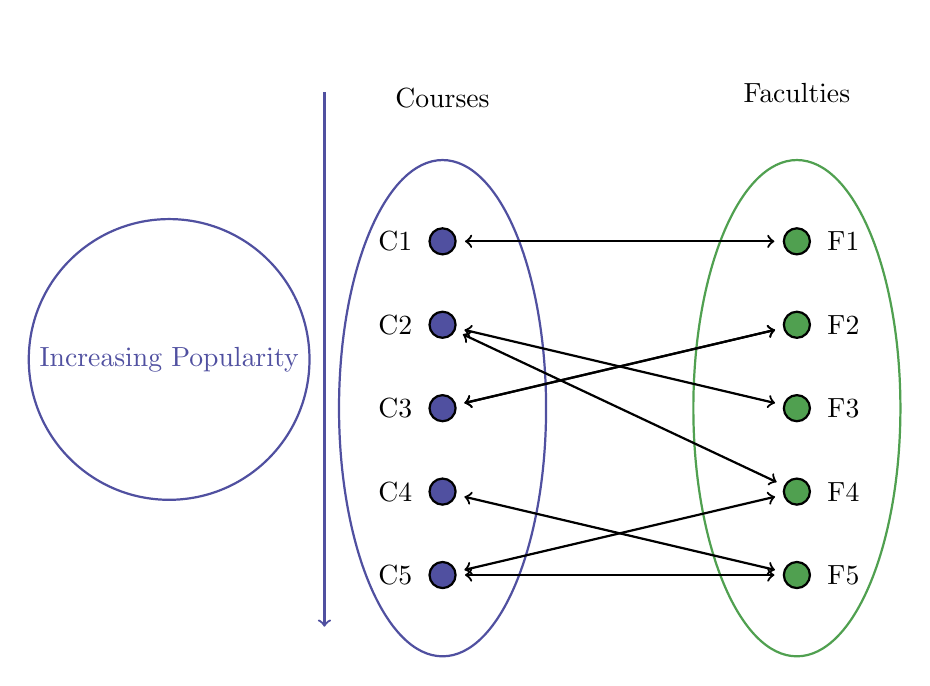
\begin{tikzpicture}[thick,
    every node/.style={draw,circle},
    fsnode/.style={fill=myblue},
    ssnode/.style={fill=mygreen},
    every fit/.style={ellipse,draw,inner sep=-2pt,text width=2cm},
    <->,shorten >= 3pt,shorten <= 3pt
  ]

  % the vertices of Faculty
  \begin{scope}[xshift=-0.5cm,yshift=-0.5cm,start chain=going below,node distance=7mm]
  \foreach \i in {1,2,...,5}
    \node[fsnode,on chain] (f\i) [label=left: C\i] {};
  \end{scope}

  % the vertices of Courses
  \begin{scope}[xshift=4cm,yshift=-0.5cm,start chain=going below,node distance=7mm]
  \foreach \i in {1,2,...,5}
    \node[ssnode,on chain] (s\i) [label=right: F\i] {};
  \end{scope}

  % the set Faculty
  \node [myblue,fit=(f1) (f5),label=above:Courses] {};
  % the set Courses
  \node [mygreen,fit=(s1) (s5),label=above:Faculties] {};

  % the edges
  \draw (f1) -- (s1);
  \draw (s4) -- (f2);
  \draw (f2) -- (s3);
  \draw (s2) -- (f3);
  \draw (s5) -- (f4);
  \draw (f3) -- (s2);
  \draw (s4) -- (f5);
  \draw (f5) -- (s5);
  \draw[->,myblue, thick] (-2,1.5) -- (-2,-5.5) node[midway, left=5pt, align=center]{Increasing Popularity};
  \end{tikzpicture}
  \caption{Faculty-Course Assignment.}



\end{figure}
\index{Algorithmic Approach}
\section{Algorithmic Approach}

Our algorithm initiates with a bipartite unidirectional graph, modeling the relationship between faculty members and courses, with courses initially assigned to faculties. The objective is to construct an initial solution through a partially greedy procedure. A key element of this approach is the utilization of a popularity function.

The popularity function is defined for both faculty members and courses. A higher popularity for a course indicates it is more favored among faculty members. The calculation involves the preference list, where, for example, if a course appears second in the preference list of a faculty, the added popularity is determined by the total number of courses in that preference list and the position of the course in the preference list of the faculty (shown as an equation below).

\begin{equation}
\text{Popularity of a course} = \sum_{i} (n_i - y_i + 1)
% \text{Popularity of a course} = \text{Total courses in preference list} - \text{their position in the preference list of }
\end{equation}
\begin{align*}
&\text{where} \\
&n_i : \text{Number of unique courses in the preference list of all the faculties.} \\
&y_i : \text{Position of the course in the preference list of the } i\text{-th faculty. If the course isn't present,} \\
&\text{it is given the } (n_i + 1)\text{-st position.}
\end{align*}
Similarly, for faculty members, the popularity is the sum of the popularity values of all courses in their preference list. The faculties and courses are then sorted in ascending order based on their popularity.

Subsequently, an iteration is performed through courses and, within that, through faculties. Courses are assigned to faculties if the course exists in their preference list and there are sufficient credits remaining. This process results in an initial solution.

To introduce randomness and explore alternative solutions, the initial solution undergoes a random change. This is achieved through a local search mechanism, identifying positions where two courses of equal popularity can be exchanged.


The algorithm performs efficiently even for extensive test cases due to its O(nlogn) time complexity. Consequently, it effectively transforms this NP-hard problem into a P-hard solution.

\newpage
\index{Pseudocode}
\section{Pseudocode}
\begin{algorithm}
\caption{Generate Initial Solution}
\KwData{graph}
\While{reading input}{
    \texttt{calculatePopularity(graph)}\;
    \texttt{sortFacultiesByPopularity()}\;
    \texttt{sortCoursesByPopularity()}\;
    \For{\texttt{each course in courses}}{
        \For{\texttt{each faculty in faculties}}{
            \If{\texttt{course in faculty.preferenceList and faculty.hasSufficientCredits(course)}}{
                \texttt{assignCourseToFaculty(course, faculty)}\;
            }
        }
    }
    \texttt{introduceRandomness()}\;
    \texttt{localSearch()}\;
}
\end{algorithm}
% \newpage
\index{Input-Output}
\section{Input-Output}
The input is in the form of a CSV File of the folllowing format : \\
    Column 1 : Professor name \\
    Column 2 : Array of UGCDC choices \\
    Column 3 : Array of UGELECT choices \\
    Column 4 : Array of HDCDC choices\\
    Column 5 : Array of HDELECT choices \\
    Column 6 : Professor category (x1, x2, x3) \\
    
Do note that the arrays contain the indexes of the courses, the course name corresponding to each index can be found in the code.

    
\newpage
\index{Test Cases}
\section{Test Cases}

\begin{table}[h]
  \centering
  \caption{Professor Course Preferences}
  \begin{tabular}{lcccccc}
    \toprule
    Name & UGCDC & UGELEC & HDCDC & HDELEC & Category \\
    \midrule
       Snehanshu Saha & 4 5 3 7 & 2 0 1 6 & 2 3 0 4 & 3 1 2 4 & x3 \\
Ramprasad S. Joshi & 0 1 2 8 & 2 3 0 4 & 3 1 2 & 1 2 3 & x1 \\
Harikrishnan N. B. & 2 3 1 6 & 3 1 2 4 & 3 2 1 & 2 0 1 & x2 \\
A. Baskar & 1 3 2 4 & 1 3 0 5 & 3 1 2 4 & 1 2 3 4 & x3 \\
Aditya Challa & 2 3 0 9 & 3 1 2 5 & 2 3 0 & 2 0 1 4 & x2 \\
Arnab Kumar Paul & 0 1 2 5 & 2 3 1 5 & 3 1 2 & 1 2 3 & x3 \\
Ashwin Srinivasan & 1 3 0 4 & 3 1 2 6 & 3 2 1 & 2 5 0 1 & x3 \\
Biju K. Raveendran Nair & 0 1 3 6 & 2 3 0 4 & 2 3 0 & 1 2 6 3 & x2 \\
Devashish Gosain & 1 2 3 & 1 2 3 4 & 3 2 0 & 3 0 1 & x2 \\
Sougata Sen & 2 3 1 & 3 1 2 3 & 3 2 1 & 2 0 1 & x2 \\
Hemant Rathore & 1 3 2 & 1 3 0 4 & 3 1 2 4 & 1 2 3 & x3 \\
Basabdatta Bhattacharya & 2 3 0 & 3 1 2 5 & 2 3 0 & 2 0 1 & x2 \\
Bharat Madhusudan Deshpande & 0 1 2 & 2 3 0 6 & 3 1 2 & 6 1 2 3 & x3 \\
Diptendu Chatterjee & 1 3 0 & 3 1 2 5 & 3 2 1 & 2 0 1 & x3 \\
Kanchan Manna & 0 1 2 & 2 3 0 6 & 3 1 2 & 1 2 3 & x3 \\
Kunal Kishore Korgaonkar & 2 3 1 & 3 1 2 & 3 2 1 4 & 2 0 1 & x2 \\
Neena Goveas & 1 3 2 & 1 3 0 & 3 1 2 & 1 2 3 & x3 \\
Rajesh Kumar & 0 1 2 & 2 3 0 & 3 1 2 & 1 2 3 & x3 \\
Santonu Sarkar & 2 3 1 & 3 1 2 & 3 2 1 & 2 0 1 & x2 \\
Vinayak Naik & 1 2 3 & 1 2 3 & 3 2 0 4 & 3 0 1 & x2 \\
Sujith Thomas & 0 1 2 & 2 3 0 & 3 1 2 & 5 1 2 3 & x2 \\
Swaroop Joshi & 2 3 0 & 3 1 2 & 2 3 0 & 2 0 1 4 & x2 \\
Swati Agarwal & 1 3 2 & 1 3 0 & 3 1 2 & 1 2 3 & x3 \\
Tanmay Tulsidas Verlekar & 2 3 1 & 3 1 2 & 3 2 1 & 5 2 0 1 & x2 \\

    \bottomrule
  \end{tabular}
  \label{tab:prof_preferences}
\end{table}


\subsection{Test Case 1}
\begin{lstlisting}[basicstyle=\ttfamily\footnotesize, breaklines=true]
Output: 1

1. Ramprasad S. Joshi
    1. CS F342 CompArch
2. Aditya Challa
    1. CS F351 ToC
3. Snehanshu Saha
    1. CS F301 PoPL
    2. CS C623 Advanced Operating Systems
4. Swaroop Joshi
    1. CS G513 Network Security
    2. CS G525 Advanced Computer Networks
5. Basabdatta Bhattacharya
    1. CS G513 Network Security
    2. CS G525 Advanced Computer Networks
6. Biju K. Raveendran Nair
    1. CS F215 DD
    2. CS F11 CP1
7. Sujith Thomas
    1. CSG524 Advanced Computer Architecture
    2. CS F11 CP1
8. Diptendu Chatterjee
    1. CS G526 Advanced Algorithms and Complexity
    2. CS F214 LCS
    3. CS F12 CP2
9. Ashwin Srinivasan
    1. CS F222 DisCo
    2. CS F214 LCS
    3. CS F12 CP2
10. Bharat Madhusudan Deshpande
    1. SS G554 Distributed Data Systems
    2. BITS F463 CRYPTOGRAPHY
11. A. Baskar
    1. CS F222 DisCo
    2. SS G513 Network Security
12. Hemant Rathore
    1. BITS F386 QUANTUM INFO & COMPUTING
13. Arnab Kumar Paul
    1. CS F213 OOP
    2. BITS F452 BLOCKCHAIN TECHNOLOGY
14. Tanmay Tulsidas Verlekar
    1. CS G523 Software for Embedded Systems
15. Rajesh Kumar
    1. CSG524 Advanced Computer Architecture
    2. CS G526 Advanced Algorithms and Complexity
    3. BITS F311 Image Processing
16. Devashish Gosain
    1. BITS F386 QUANTUM INFO & COMPUTING
    2. SS G527 Cloud Computing
17. Vinayak Naik
    1. CS C623 Advanced Operating Systems
    2. SS G527 Cloud Computing
    
18. Kanchan Manna
    1. BITS F463 CRYPTOGRAPHY
    2. BITS F311 Image Processing
    3. CS G568 Network Security Projec
19. Sougata Sen
    1. CS F13 CP3
    2. BITS F343 FUZZY LOGIC & APPL
20. Santonu Sarkar
    1. CS F13 CP3
    2. BITS F343 FUZZY LOGIC & APPL
21. Harikrishnan N. B.
    1. CS F215 DD
    2. CS G553 Reconfigurable Computing
22. Neena Goveas
    1. CS G568 Network Security Projec
    2. BITS F312 NEURAL NET & FUZZY LOGIC
    3. BITS G553 Real-Time Systems
23. Kunal Kishore Korgaonkar
    1. CS G553 Reconfigurable Computing
    2. BITS F364 HUMAN COMP INTERACTION
24. Swati Agarwal
    1. BITS F312 NEURAL NET & FUZZY LOGIC
    2. BITS G553 Real-Time Systems
    3. BITS F364 HUMAN COMP INTERACTION

Total Number of Courses Assigned is: 27

... (further outputs) ...

Time efficiency : 304 outputs in 0.0202256 seconds

\end{lstlisting}

In this particular scenario, the algorithm successfully assigned 27 out of the 29 available courses, taking into account the individual course preferences and categories specified by each faculty member. The assignments were tailored to match the unique preferences and categories of each professor, ensuring a comprehensive distribution of courses.


\subsection{Test Case 2}

INPUT : 
\begin{table}[h]
  \centering
  \caption{Professor Course Preferences}
  \begin{tabular}{lcccccc}
    \toprule
    Name & UGCDC & UGELEC & HDCDC & HDELEC & Category \\
    \midrule
        A. Baskar & 1 3 2 4 & 1 3 0 5 & 3 1 2 4 & 1 2 3 4 & x3 \\
    Aditya Challa & 2 3 0 9 & 3 1 2 5 & 2 3 0 & 2 0 1 4 & x2 \\
    Arnab Kumar Paul & 0 1 2 5 & 2 3 1 5 & 3 1 2 & 1 2 3 & x3 \\
    Ashwin Srinivasan & 1 3 0 4 & 3 1 2 6 & 3 2 1 & 2 5 0 1 & x3 \\
    Biju K. Raveendran Nair & 0 1 3 6 & 2 3 0 4 & 2 3 0 & 1 2 6 3 & x2 \\
    \\
    \bottomrule
  \end{tabular}
  \label{tab:prof_preferences}
\end{table}
  \\
OUTPUT : 
\\
\begin{lstlisting}[basicstyle=\ttfamily\footnotesize, breaklines=true]


(Terminating Program)
CRASH TEST: NO PROFESSOR HAS TAKEN COURSE CS F301 PoPL


\end{lstlisting}
\index{Crash Test}
\section{Crash Test}

The algorithm concludes its execution under two conditions: either when all assignments are successfully completed, or when it identifies an impractical scenario where no feasible assignment aligns with both the professors' preference lists and the hard constraints. To be more specific, termination occurs in the following scenarios:

1. If there are UGCDCs that remain unchosen by any professor.

2. If there are HDCDCs that remain unchosen by any professor.

Under these circumstances, the algorithm returns the course that is unchosen and terminates.
\index{Consistency Report}
\section{Consistency Report}

To evaluate the consistency of the algorithm, we define the following metrics and criteria:

\begin{itemize}
    \item \textbf{Accuracy:} The correctness of the assignments made by the algorithm is 100\% as each assignment makes sure that the faculty category and preference order are taken care of and also that a course is completely assigned.
    \item \textbf{Precision:} The algorithm gives multiple solutions out of which most of the first few outputs will always be sub-optimal solutions of the problem.
\end{itemize}

The input format for the algorithm is the preference order of faculty for the courses they decide to teach, and the output is the assignment of faculty with consideration for their category constraints. Additionally, the algorithm ensures that a course is not assigned partially.


\index{Future Possible Extensions}
\section{Future Possible Extensions}

\subsection{Genetic Algorithm Integration:}
The algorithm's capabilities can be further extended by incorporating a genetic algorithm paradigm. Post the initial assignment, the introduction of fitness, mutate, and crossover functions within a genetic algorithm framework can enhance the optimization process, potentially leading to improved solutions.

\subsection{Generalization for Diverse Professor Categories:}
The algorithm's adaptability can be further demonstrated by extending its functionality to accommodate a broader spectrum of professor categories. This generalization would enhance its utility across various academic scenarios, allowing for more inclusive and flexible assignment solutions.

\subsection{Application in Other Operations Research Problems:}
Leveraging the algorithm's effectiveness in solving the course faculty assignment problem, it can be applied to address additional Operations Research problems like Employee shift scheduling, Exam Scheduling,etc. Its versatility can potentially streamline solutions for problems beyond academic scheduling, showcasing its applicability in diverse operational scenarios.

\subsection{Development of User-Friendly Software:}
A comprehensive software solution can be developed with a user-friendly frontend interface. This software would serve as a practical tool for faculties to submit their preferences and for Head of Departments (HODs) to efficiently assign courses. This integration of technology can enhance user experience, making the entire assignment process more accessible and intuitive.

By exploring these future extensions, the algorithm not only expands its scope and applicability but also contributes to the development of advanced solutions in the field of academic scheduling and beyond.
\index{References}
\section*{References}
\begin{enumerate}
    \item Andres Ramos and Tomas Santero, ``The biquadratic assignment problem: A new mathematical programming model and computational results,'' \textit{Reliability Engineering \& System Safety}, vol. 189, pp. 106823, 2019. DOI: \url{https://www.sciencedirect.com/science/article/pii/S0305054819300486}

    \item A. A. Popov et al, ``A GRASP for the biquadratic assignment problem,'' \textit{Journal of Physics: Conference Series}, 2020.

    \item Author Name, ``A GRASP for the biquadratic assignment problem,'' Year. \url{https://www.academia.edu/2933036/A_GRASP_for_the_biquadratic_assignment_problem}
\end{enumerate}

\printindex
\end{document}